\begin{frame}{Representações sucintas de árvores}
    \textbf{Representação de árvores sucintas via Parênteses Balanceados}
        \begin{figure}[h!]
            \centering
            
            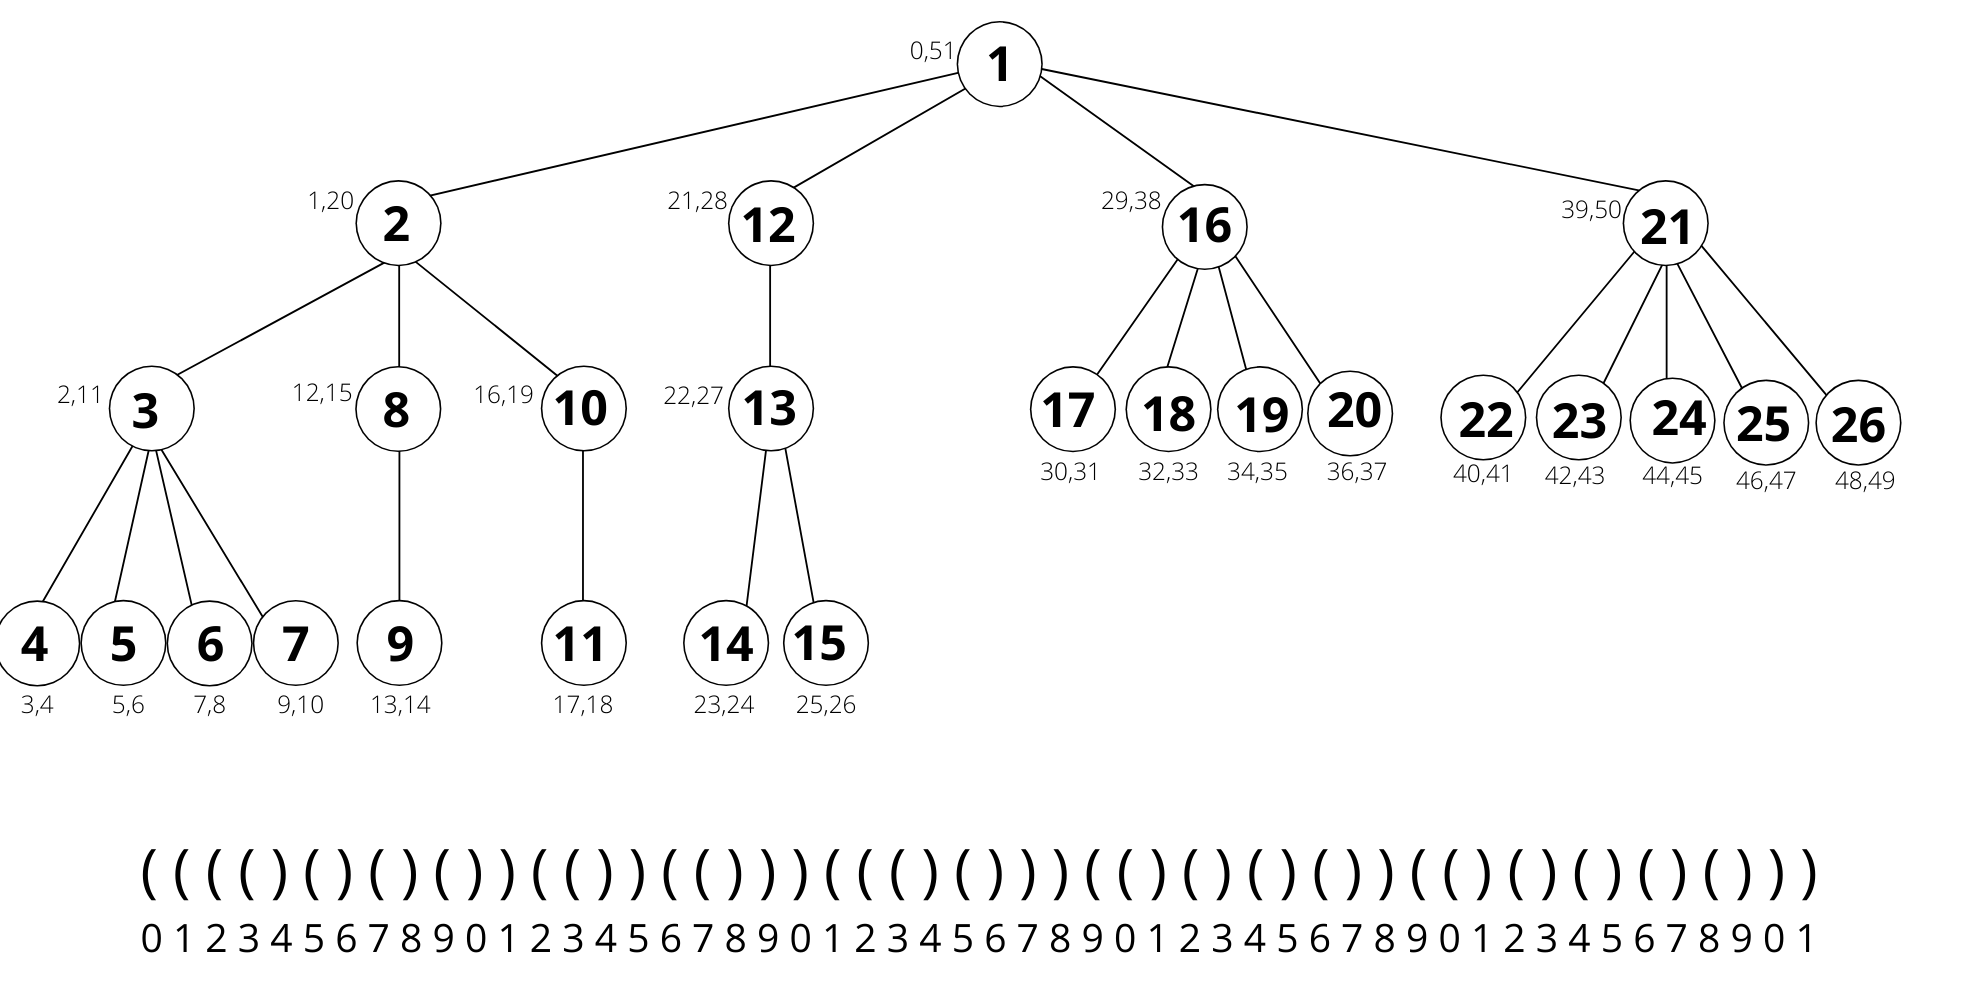
\includegraphics[scale=0.37]{images/arvore_geral.png}
        \end{figure} 
\end{frame}

\begin{frame}{Representações sucintas de árvores}
    \textbf{Representação de árvores sucintas via parênteses balanceados}
        \begin{itemize}
            \item Sequência de $2n$ parênteses balanceados;
            \item Complexidade de espaço $2n$ bits;
            \item Através de estruturas auxiliares suporta:
            \begin{itemize}
                \item findclose(BP,i);
                \item findopen(BP,i);
                \item excess(BP,i);
            \end{itemize}
        \end{itemize}
    \end{frame}
    
    \begin{frame}{Representações sucintas de árvores}
    Exemplo: \textit{excess(BP,6) = -1}
        \begin{figure}[h!]
            \centering
            
            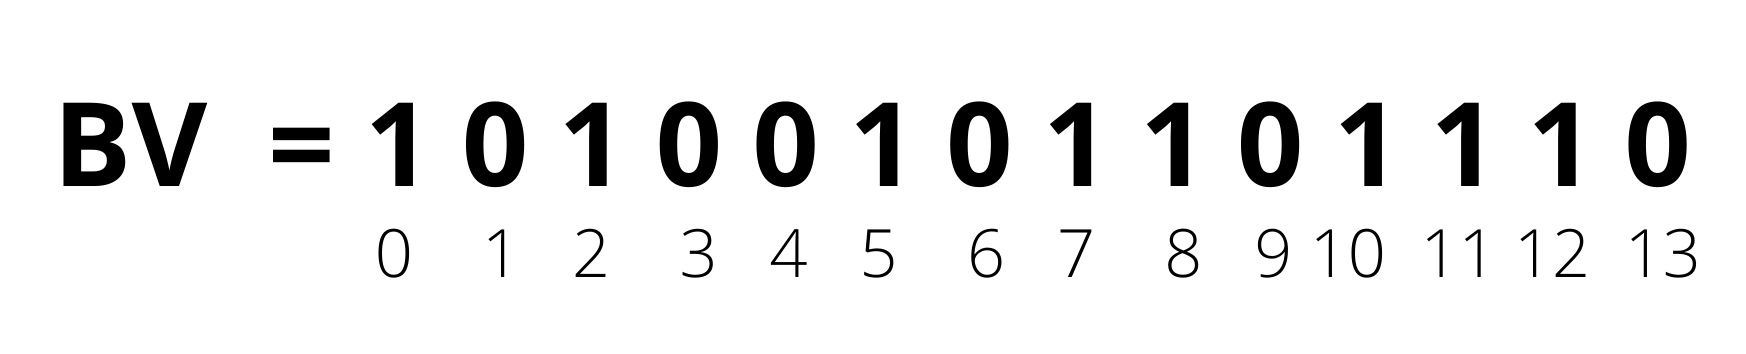
\includegraphics[scale=0.5]{images/bitvector.png}
        \end{figure} 
\end{frame}